\documentclass[a4paper]{article}

%% Language and font encodings
\usepackage[english]{babel}
\usepackage[utf8x]{inputenc}
\usepackage[T1]{fontenc}

%% Sets page size and margins
\usepackage[a4paper,top=3cm,bottom=2cm,left=3cm,right=3cm,marginparwidth=1.75cm]{geometry}

%% Useful packages
\usepackage{amsmath}
\usepackage{graphicx}
\usepackage{textpos}
\usepackage{float}
\usepackage[colorinlistoftodos]{todonotes}
\usepackage[colorlinks=true, allcolors=black]{hyperref}
\usepackage[numbered,framed]{matlab-prettifier}
\usepackage{relsize}
\usepackage{amsmath}
\usepackage{amssymb}
\usepackage{amsthm}

%% Package for graphs
\usepackage{tikz}

%% Package for loading MatLab
\usepackage[framed,numbered,autolinebreaks,useliterate]{mcode}

\setlength{\parindent}{0pt}
\newcommand{\p}{\mathbb{P}}

\title{\vspace*{2cm}9.5 The Google PageRank Algorithm\vspace*{-1.5cm}}
\date{}

\begin{document}
\maketitle

\begin{textblock*}{100mm}(0cm,-5.5cm)
\Huge 9.5
\end{textblock*}

\section*{The PageRank Algorithm}
\subsection*{Question 1}

Consider the following adjacency matrix $A$ and corresponding transition matrix $S$ for the directed graph included in figure \ref{fig:q1}. The recursion iterating with $S$ fails to converge when initialised with $w=(1,1,1)$, instead it produces a repeating 2-cycle with $Aw \neq w$ and $A^2w = w$ which can be seen as follows:

\begin{equation*}
    A = \begin{pmatrix}
        0 & 1 & 1 \\
        1 & 0 & 0 \\
        1 & 0 & 0 
    \end{pmatrix}
    \qquad \Longrightarrow \qquad 
    S = \begin{pmatrix}
          0 & 1 & 1 \\
        1/2 & 0 & 0 \\
        1/2 & 0 & 0 
    \end{pmatrix}
\end{equation*}

\begin{align*}
    w = \begin{pmatrix} 1 \\ 1 \\ 1 \end{pmatrix}
    \qquad
    Aw = \begin{pmatrix} 2 \\ 1/2 \\ 1/2 \end{pmatrix}
    \qquad
    A^2w = \begin{pmatrix} 1 \\ 1 \\ 1 \end{pmatrix}
\end{align*}

\begin{figure}[H]
    \centering
    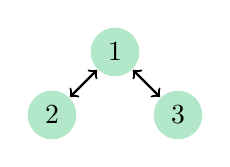
\begin{tikzpicture}
        [scale=.8,auto=left,thick,every node/.style={circle,fill=blue!30!green!30}]
        \node (A) at (2,2) {1};
        \node (B) at (1,1) {2};
        \node (C) at (3,1) {3};
        
        \path [<->] (A) edge (B);
        \path [<->] (A) edge (C);
    
    \end{tikzpicture}
    \caption{A directed graph described by the adjacency matrix $A$}
    \label{fig:q1}
\end{figure}

\subsection*{Question 2}
Script Q2.m (pg.\pageref{PQ2}) simulates 100 sample paths of the Markov chain defined by the 'Random Surfer' Method on the graph (drawn in figure \ref{fig:q2}) described by the adjacency matrix $A$ with $\pi$ uniform and $d=0.85$.

\begin{equation*}
    A = \begin{pmatrix}
        0 & 1 & 0 & 0 \\
        1 & 0 & 0 & 0 \\
        1 & 0 & 0 & 1 \\
        0 & 0 & 0 & 0
    \end{pmatrix}
    \qquad
    \pi = \begin{pmatrix} 1/4 \\ 1/4 \\ 1/4 \\ 1/4 \end{pmatrix}
    \qquad
    d = 0.85
\end{equation*}

\begin{figure}[H]
    \centering
    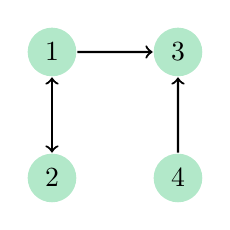
\begin{tikzpicture}
        [scale=.8,auto=left,thick, every node/.style={circle,fill=blue!30!green!30}]
        \node (A) at (0,2) {1};
        \node (B) at (0,0) {2};
        \node (C) at (2,2) {3};
        \node (D) at (2,0) {4};
        
        \path [<->] (A) edge (B);
        \path [->] (A) edge (C);
        \path [->] (D) edge (C);
    
    \end{tikzpicture}
    \caption{A directed graph described by the adjacency matrix $A$}
    \label{fig:q2}
\end{figure}

Script Q2.m produces two graphs. Firstly, a graph of $\mu_{jt}^{(k)}$, the average time spent on the $k$th node from the beginning of the sample path until time $t$, against time, $t$, for $j$ fixed is shown in figure \ref{fig:q2a}. A sample of the beginning of the path is included below and figure \ref{fig:q2aa} includes the average time spent at each node by the end of the fixed path (this is included for future reference in the project). Secondly, figure \ref{fig:q2} is a graph of the variance, $Var(\mu_{jt}^{(k)})$, against $t$ for each node $k$.
\begin{equation*}
    path = \begin{matrix} 1,\ 3,\ 4,\ 3,\ 4,\ 3,\ 4,\ 3,\ 1,\ 2,\ 1,\ 2,\ 1,\ 3,\ 2,\ ... \end{matrix}
\end{equation*}

\begin{figure}[H]
    \centering
    \begin{verbatim}
                fix_path_mu =
                    0.3160    0.2280    0.3560    0.1000
    \end{verbatim}
    \caption{The average time spent at each node by the end of the fixed path plotted in figure \ref{fig:q2a}.}
    \label{fig:q2aa}
\end{figure}

\begin{figure}[H]
    \centering
    \includegraphics[width=\columnwidth]{q2.png}
    \caption{A graph of $\mu_{jt}^{(k)}$ against $t$ for all $k$ generated by script Q2.m.}
    \label{fig:q2a}
\end{figure}

\begin{figure}[H]
    \centering
    \includegraphics[width=\columnwidth]{q2var.png}
    \caption{A graph of $Var(\mu_{jt}^{(k)})$ against $t$ for all $k$ generated by script Q2.m.}
    \label{fig:q2b}
\end{figure}

\subsection*{Question 3}

To incorporate damping and dangling nodes as described by the Random Surfer method we modify the transition matrix described in question 1 to be as follows:
\begin{equation*}
    w_i = \sum^N_{j=1}S_{ij}w_j
\end{equation*}
\begin{equation*}
    S_{ij} = \begin{cases}
        \frac{A_{ij}}{\sum_{q=1}^N A_{qj}}\times d + \pi_i \times (1-d) & \text{for } \sum_{q=1}^N A_{qj} > 0 \\
        \qquad \pi_i & \text{otherwise}
    \end{cases}
\end{equation*}

\subsubsection*{Standard result from Markov Chains}
A Markov chain that is irreducible, aperiodic and positive recurrent has
\begin{align*}
    p_{i,j}(n) \rightarrow \pi_j = \frac{1}{\mu_j}
\end{align*}
as $n\rightarrow \infty$, where $\pi$ is the unique invariant distribution and $\mu_i$ is the mean recurrence time of $i$.

\bigskip
The new modified recursion is irreducible, aperiodic and positive recurrent. This is due to the damping meeting the condition, $\pi_i > 0$, meaning at any step it is possible to move to any vertex from any vertex in a single step. Consequently:
\begin{itemize}
    \item
    there is only one communicating class $\Rightarrow$ irreducible
    \item
    $p_{i,i}(1) > 0$ for all $i$ $\Rightarrow$ aperiodic
    \item
    $\mathbb{P}_i(T_i>n) \rightarrow 0$ as $n \rightarrow \infty$ giving $\mathbb{P}_i(T_i<\infty) = 1$ $\Rightarrow$ positive recurrent
\end{itemize}

Therefore, by the quoted result the recursion converges to a unique solution, $p$, which is a distribution. We note that $\mu_i$ being the mean recurrence time of $i$ implies that $p_i$ represents the average time spent at $i$, or in our case the average time the surfer spends visiting webpage $i$.

\subsection*{Question 4}

Script PageRank.m (pg.\pageref{PPageRank}) is a funciton which implements the PageRank method. It accepts the following inputs:
an adjacency matrix, $A$, a distribution for choosing a random webpage, $\pi$, a damping probability, $d$, and a maximum number of iterations. It returns a column vector, $w$, of PageRank scores.

\bigskip
Script Q4a.m (pg.\pageref{fig:q4a}) is a short script which applies this method to the case described in question 2 with $\pi$ uniform and $d=0.85$. The PageRank generated is included in figure \ref{fig:q4a}.
\begin{figure}[H]
    \centering
    \begin{minipage}[b]{0.45\linewidth}
        \centering
        \begin{verbatim}
            w =
                1.2581
                0.9691
                1.3383
                0.4344
                
        \end{verbatim}
        \caption{PageRank generated with script Q4a.m for $A$ as given in question 2.}
        \label{fig:q4a}
    \end{minipage}
    \hfill
    \begin{minipage}[b]{0.45\linewidth}
        \centering
        \begin{verbatim}
            w =
                0.4344
                1.8713
                0.3346
                0.3346
                2.0250
        \end{verbatim}
        \caption{PageRank generated with script Q4b.m for $A$ as in figure \ref{fig:q4bb}}
        \label{fig:q4b}
    \end{minipage}
\end{figure}

In question 3 we discussed how the limit of the recursion of the PageRank algorithm is a distribution which represents the average time the surfer spends visiting each webpage, this is exactly what we calculated in question 2. Therefore by considering $p=w/N$ we can compare results (see figure \ref{fig:q4aa}) and see that they agree very strongly.
\begin{figure}[H]
    \centering
    \begin{verbatim}
        fix_path_mu =
            0.3160    0.2280    0.3560    0.1000
        p =
            0.3145    0.2423    0.3346    0.1086
    \end{verbatim}
    \caption{Comparison of the average time spent at each node by the fixed path recorded in question 2 (top) with $p=w/N$ as calculated by script Q4a.m (bottom).}
    \label{fig:q4aa}
\end{figure}

We note that the PageRank algorithm can produce some surprising results. Consider the following example in which a node, node 1, has more incoming and outgoing links than another node, node 2, but receives a lower score of 0.4344 compared to 1.8713. The full PageRank for this example is included in figure \ref{fig:q4b}.
\begin{figure}[H]
    \centering
    \begin{minipage}[b]{0.48\linewidth}
        \centering
        \begin{equation*}
            A = \begin{pmatrix}
                0 & 0 & 1 & 1 & 0 \\
                0 & 0 & 0 & 0 & 1 \\
                1 & 0 & 0 & 0 & 0 \\
                1 & 0 & 0 & 0 & 0 \\
                0 & 1 & 1 & 1 & 0 \\
            \end{pmatrix}
            \vspace{0.5pt}
        \end{equation*}
    \end{minipage}
    \hfill
    \begin{minipage}[b]{0.48\linewidth}
        \centering
        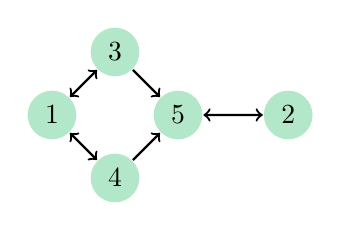
\begin{tikzpicture}
            [scale=.8,auto=left,thick,every node/.style={circle,fill=blue!30!green!30}]
            \node (A) at (0,1) {1};
            \node (B) at (1,2) {3};
            \node (C) at (1,0) {4};
            \node (D) at (2,1) {5};
            \node (E) at (3.75,1) {2};
            
            \path [<->] (A) edge (B);
            \path [<->] (A) edge (C);
            \path [->] (B) edge (D);
            \path [->] (C) edge (D);
            \path [<->] (D) edge (E);
        \end{tikzpicture}
    \end{minipage}
    \caption{An example graph with node 1 having both more incoming and outgoing links than node two, but a smaller PageRank score.}
    \label{fig:q4bb}
\end{figure}


\subsubsection*{Question 5}
Script RandWebRank.m (pg.\pageref{PQ5rand}) generates a random adjacency matrix of size N such that the out-degree of each node is an independent Poisson random variable with a mean $k$ and conditional on the sequence of the out-degrees all graphs are equiprobable. It does this by determining the out-degree of each node in tern then randomly assigning corresponding outgoing links to other pages. Then script Q5.m (pg.\pageref{PQ5}) applies and tests this function as follows.

\bigskip
To check this implementation of the PageRank algorithm is correct we can inspect the eigenvectors of the modified transition matrix, $S$. In particular the PageRank score is an eigenvector with eigenvalue 1. Therefore we can find the eigenvector of $S$ with eigenvalue 1 by an alternative method, such as the MATLAB eig function, and compare this with the PageRank scores to see if they are equal. Figure \ref{fig:q5a} includes a sample of the output from Q5.m comparing these two vectors. This comparison affirms the validity of this implementation of PageRank.
\begin{figure}[H]
    \centering
    \begin{verbatim}
        1.0644    1.0644
        1.0636    1.0636
        1.0562    1.0562
        0.8864    0.8864
        1.0443    1.0443
        0.9138    0.9138
        1.1308    1.1308
        1.0394    1.0394
        0.9921    0.9921
        0.9490    0.9490
    \end{verbatim}
    \caption{A sample of the comparison of the PageRank scores against the eigenvector of the modified transition matrix with eigenvalue 1.}
    \label{fig:q5a}
\end{figure}

\bigskip
Script Q5\_empirical.m (pg.\pageref{PQ5emp}) investigates the impact of varying $k$ on the empirical distribution by generating multiple graphs of size $N$ but with different values of $k$ and then compares them by plotting their respective empirical distributions on the same graph. Figure \ref{fig:q5b} includes a graph produced by this script from which we can see that the greater the number of links in the random network of webpages then the tighter the rankings. This is to be expected because on average more links per node leads to a smaller variance in the expected links at each node and so a more consitent graph with a closer ranking. 
\begin{figure}[H]
    \centering
    \includegraphics[width=1\columnwidth]{q5empirical.png}
    \caption{A graph comparing the empirical distribution of PageRank scores for decreasing values of $k$ from 100 to 5.}
    \label{fig:q5b}
\end{figure}

\bigskip
An aspect of this model which provides an unrealistic description of real-life networks is the equal probability of all graphs conditional on a given sequence of out-degrees. In real life there is likely to be some form of correlation between links. We expect there to be some key websites which a lot of websites link to and then smaller websites that very few websites link to.

\subsection*{Question 6}

Script Journals.m (pg.\pageref{Pjournals}) processes the data from data files \texttt{citations.dat} and \texttt{articlejids.dat}. It verifies that the same set of articles appears in both files and that a unique journal identifier is given to every article (see figure \ref{fig:q6}). It then converts the two data sets into an adjacency matrix A between journals and also a vector $z$ of articles per journal.
\begin{figure}[H]
    \centering
    \begin{verbatim}
        same_articles =
          logical
           1
        
        all_jids_unique =
          logical
           1
    \end{verbatim}
    \caption{Output from Journals.m verifying the same set of articles appears in both files and that a unique journal identifier is given to every article.}
    \label{fig:q6}
\end{figure}

\subsubsection*{Question 7}

Script Journals.m also computes the Eigenfactor (EF) and Total Citations (TC) scores. From this it then determines the correlation between the two. The correlation is 0.9908 (see figure \ref{fig:q7cor}) which is a very strong correlation and makes a strong case that these two schemes are practically indistinguishable.

\begin{figure}[H]
    \centering
    \begin{verbatim}
        rhoEFTC =
            0.9908
    \end{verbatim}
    \caption{Correlation between Eigenfactor (EF) and Toal Citaitons (TC) scores.}
    \label{fig:q7cor}
\end{figure}

Figure \ref{fig:q7rank} compares the top rankings according to the EF and TC scoring methods. Once scores have been converted to rankings we can see that EF and TC are very similar and differences are very negligible amongst the highest scoring journals. Furthermore considering that the top end of the rankings represents the most valuable data this further supports the claim that they are practically indistinguishable.
\begin{figure}[H]
    \centering
    \begin{verbatim}
        EF    TC
        82    82
       270   270
        90    90
        55    55
       173   173
        95    84
        84    95
        64    64
        42    42
        71    71
        12    12
        68   256
       256    68
       161    79
        79   161
    \end{verbatim}
    \caption{Comparison of the top 15 ranked journals according to Eigenfactor (EF) and Toal Citaitons (TC) scores.}
    \label{fig:q7rank}
\end{figure}

For further comparison figure \ref{fig:q7graph} graphs the rankings of each journal according to the two scoring systems. This gives us a visual sense of how the scoring systems compare. This provides some further information which suggests that the systems also score very low ranking pages very similarly too. It is the mid-range journals which receive the most variable ranking and this is to be expected because in the middle of the pack journals are receiving very similar scores and so ranking amplifies very small variations in score. These observations match closely with the empirical distributions looked at in question 5.
\begin{figure}
    \centering
    \includegraphics[height=1.5\columnwidth]{q7.png}
    \caption{A graph comparing the rankings of journals according to the EF and TC scoring systems. The graph is scoring system (x-axis) against ranking (y-axis) with each line representing a journal.}
    \label{fig:q7graph}
\end{figure}

\bigskip
Script Journals.m further computes the Article Influence (AI) and Impact Factor (IF), from EF and TC respectively, and then the correlation between the two. This correlation provides further information because we see that this correlation is marginally even stronger. AI and IF both seek to compensate for journal size, therefore this higher correlation suggests that one of EF and TC favours larger journals compared to the other.
\begin{figure}[H]
    \centering
    \begin{verbatim}
        rhoAIIF =
            0.9948
    \end{verbatim}
    \caption{Correlation between Artificial Influence (AI) and Impact Factor (IF) scores.}
    \label{fig:q7cor2}
\end{figure}

Therefore, we conclude that there is a strong case to argue that EF and TC scores are practically indistinguishable.

\pagebreak
\section*{Programs}

\subsection*{Q2.m}\label{PQ2}
\lstinputlisting{Q2.m}

\subsection*{PageRank.m}\label{PPageRank}
\lstinputlisting{PageRank.m}

\newpage
\subsection*{Q4a.m}\label{PQ4a}
\lstinputlisting{Q4a.m}

\subsection*{Q4b.m}\label{PQ4b}
\lstinputlisting{Q4b.m}

\subsection*{Q5.m}\label{PQ5}
\lstinputlisting{Q5.m}

\newpage
\subsection*{RandWebRank.m}\label{PQ5rand}
\lstinputlisting{RandWebRank.m}

\subsection*{Q5\_empirical.m}\label{PQ5emp}
\lstinputlisting{Q5_empirical.m}

\newpage
\subsection*{Journals.m}\label{Pjournals}
\lstinputlisting{Journals.m}

\end{document}
